\documentclass[a4paper]{article}

\usepackage[english]{babel}
\usepackage[utf8]{inputenc}
\usepackage{amsmath}
\usepackage{graphicx}
\usepackage{minted}
\usepackage{algorithm}
\usepackage[noend]{algpseudocode}
\usepackage[colorinlistoftodos]{todonotes}
\usepackage{multirow}
\usepackage{parskip}

% empty set package
\usepackage{amssymb}

% Automata package
\usepackage{pgf,tikz}
\usetikzlibrary{shapes,arrows,automata}


\title{CSCE 828 - Homework 2}
\author{Tian Gao}
\begin{document}
\maketitle

% Question 1
1.(a) \\
let $\Sigma = (0 \cup 1)$ \\
solution = $0 (\Sigma \Sigma)^{*} \cup 1 \Sigma (\Sigma \Sigma)^{*}$\\
1.(b)\\
let $\Sigma = (0 \cup 1)$ \\
solution = $\varepsilon \cup 1 \cup 111 \cup 0 \Sigma^{*} \cup 10 \Sigma^{*} \cup 110 \Sigma^{*} \cup 1110 \Sigma^{*} \cup 11110 \Sigma^{*} \cup 11111 \Sigma^{*}$\\
1.(c)\\
solution = $0^+0^+ \cup 10^+0^+ \cup 0^+10^+ \cup 0^+0^+1$\\

% Question 2
2. \\
step 1:\\
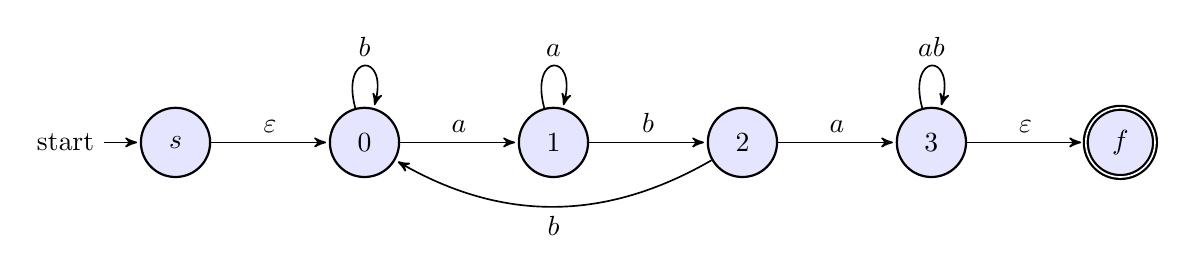
\begin{tikzpicture}[->,>=stealth',shorten >=1pt,auto,node distance=2.4cm,on grid,semithick, every state/.style={fill=blue!10,thick}]
\node[initial,state] 	 (s)              {$s$};
\node[state]        	 (0) [right of=s] {$0$};
\node[state]        	 (1) [right of=0] {$1$};
\node[state]     		 (2) [right of=1] {$2$};
\node[state]  			 (3) [right of=2] {$3$};
\node[state,accepting]   (f) [right of=3] {$f$};
\path[->] 
	(s) edge [above]        node {$ \varepsilon  $} (0)
	(0) edge [above]        node {$ a $} (1)
    (0) edge [loop above]   node {$ b $} (0)
	(1) edge [above]        node {$ b $} (2)
    (1) edge [loop above]   node {$ a $} (1)
	(2) edge [above] 		node {$ a $} (3)
	(2) edge [bend left] 	node {$ b $} (0)  
    (3) edge [loop above]   node {$ ab $} (3)
	(3) edge [above]		node {$ \varepsilon  $} (f);    
\end{tikzpicture}\\
step 2:\\
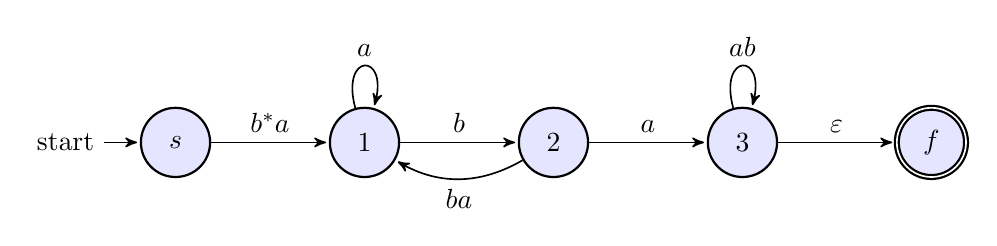
\begin{tikzpicture}[->,>=stealth',shorten >=1pt,auto,node distance=2.4cm,on grid,semithick, every state/.style={fill=blue!10,thick}]
\node[initial,state] 	 (s)              {$s$};
\node[state]        	 (1) [right of=s] {$1$};
\node[state]     		 (2) [right of=1] {$2$};
\node[state]  			 (3) [right of=2] {$3$};
\node[state,accepting]   (f) [right of=3] {$f$};
\path[->] 
	(s) edge [above]        node {$ b^*a  $} (1)
	(1) edge [above]        node {$ b $} (2)
    (1) edge [loop above]   node {$ a $} (1)
	(2) edge [above] 		node {$ a $} (3)
	(2) edge [bend left] 	node {$ ba $} (1)    
    (3) edge [loop above]   node {$ ab $} (3)
	(3) edge [above]		node {$ \varepsilon  $} (f);    
\end{tikzpicture}\\
step 3:\\
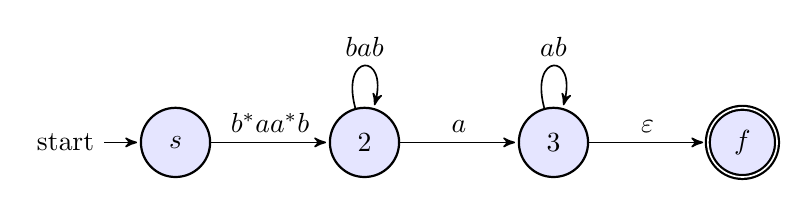
\begin{tikzpicture}[->,>=stealth',shorten >=1pt,auto,node distance=2.4cm,on grid,semithick, every state/.style={fill=blue!10,thick}]
\node[initial,state] 	 (s)              {$s$};
\node[state]     		 (2) [right of=s] {$2$};
\node[state]  			 (3) [right of=2] {$3$};
\node[state,accepting]   (f) [right of=3] {$f$};
\path[->] 
	(s) edge [above]        node {$ b^*aa^*b  $} (2)
	(2) edge [above] 		node {$ a $} (3)
	(2) edge [loop above] 	node {$ bab $} (2)   
    (3) edge [loop above]   node {$ ab $} (3)
	(3) edge [above]		node {$ \varepsilon  $} (f);    
\end{tikzpicture}\\
step 4:\\
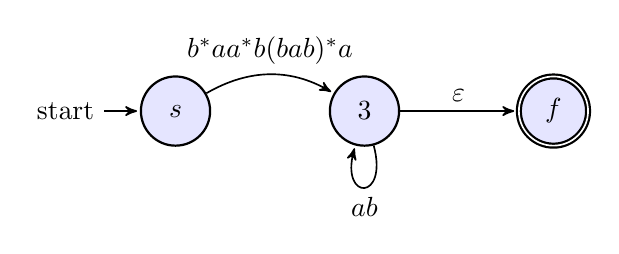
\begin{tikzpicture}[->,>=stealth',shorten >=1pt,auto,node distance=2.4cm,on grid,semithick, every state/.style={fill=blue!10,thick}]
\node[initial,state] 	 (s)              {$s$};
\node[state]  			 (3) [right of=s] {$3$};
\node[state,accepting]   (f) [right of=3] {$f$};
\path[->] 
	(s) edge [bend left]    node {$ b^*aa^*b(bab)^*a  $} (3)
    (3) edge [loop below]   node {$ ab $} (3)
	(3) edge [above]		node {$ \varepsilon  $} (f);    
\end{tikzpicture}\\
step 5:\\
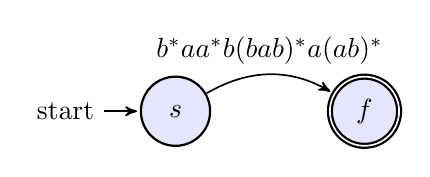
\begin{tikzpicture}[->,>=stealth',shorten >=1pt,auto,node distance=2.4cm,on grid,semithick, every state/.style={fill=blue!10,thick}]
\node[initial,state] 	 (s)              {$s$};
\node[state,accepting]   (f) [right of=s] {$f$};
\path[->] 
	(s) edge [bend left]    node {$ b^*aa^*b(bab)^*a(ab)^*$} (f);
\end{tikzpicture}\\
so solution = $ b^*aa^*b(bab)^*a(ab)^*$

% Question 3
3. \\
NFA:\\
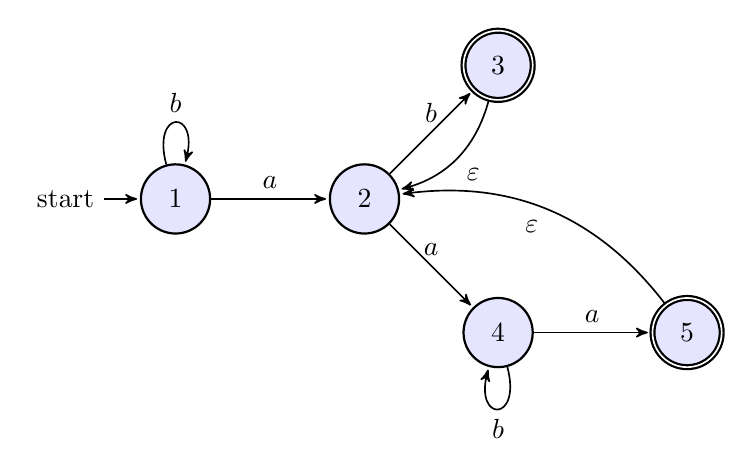
\begin{tikzpicture}[->,>=stealth',shorten >=1pt,auto,node distance=2.4cm,on grid,semithick, every state/.style={fill=blue!10,thick}]
\node[initial,state]		(1)							{$1$};
\node[state]				(2) [right of=1]			{$2$};
\node[state,accepting]		(3) [above right of=2]		{$3$};
\node[state]				(4) [below right of=2]		{$4$};
\node[state,accepting]		(5) [right of=4]			{$5$};
\path[->] 
    (1) edge [loop above]   	node {$ b $} (1)
    (1) edge [above]   			node {$ a $} (2)
	(2) edge [above] 			node {$ b $} (3)
    (3) edge [bend left] 		node {$ \varepsilon $} (2)
	(2) edge [above] 			node {$ a $} (4)  
    (4) edge [above] 			node {$ a $} (5)
    (4) edge [loop below]		node {$ b $} (4)
	(5) edge [bend right]		node {$ \varepsilon  $} (2);    
\end{tikzpicture}\\

convert NFA to DFA:\\
\begin{tabular}{|c|c|c|}
\hline
$\delta$ & a & b \\ 
\hline
\textcircled{1} & \textcircled{2} & \textcircled{1} \\
\hline
\textcircled{2} & \textcircled{4} & \textcircled{3}\textcircled{2} \\
\hline
\textcircled{4} & \textcircled{5}\textcircled{2} & \textcircled{4} \\
\hline
\textcircled{3}\textcircled{2} & \textcircled{4} & \textcircled{3}\textcircled{2} \\
\hline
\textcircled{5}\textcircled{2} & \textcircled{4} & \textcircled{3}\textcircled{2} \\
\hline
\end{tabular}\\

Min DFA:\\
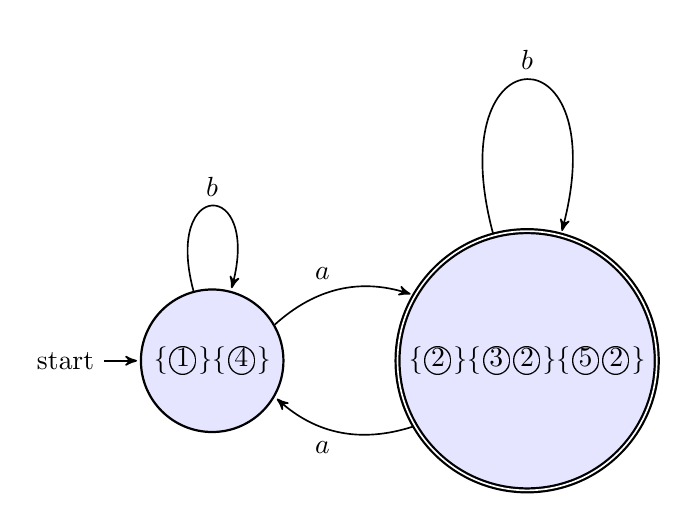
\begin{tikzpicture}[->,>=stealth',shorten >=1pt,auto,node distance=4cm,on grid,semithick, every state/.style={fill=blue!10,thick}]
\node[initial,state]				(1)							{$\{\textcircled{1}\}\{\textcircled{4}\}$};
\node[state,accepting]				(2) [right of=1]			{$\{\textcircled{2}\}\{\textcircled{3}\textcircled{2}\}\{\textcircled{5}\textcircled{2}\}$};
\path[->] 
    (1) edge [loop above]   	node {$ b $} (1)
    (1) edge [bend left]		node {$ a $} (2)
	(2) edge [bend left]		node {$ a $} (1)
    (2) edge [loop above] 		node {$ b $} (2);   
\end{tikzpicture}\\

% Question 4
4. \\
Assume that L is regular and let p be the pumping length.\\
Let $s =  " 1^pa=b+c " \in L$ where a,b,c are binary integers.\\
$\therefore |s| \geqslant p$ and $1^pa=b+c$\\
$\therefore s=xyz$ where $|y|>0$ and $|xy| < p$ (According to Pumping Lemma)\\
Let $x=1^l,y=1^m$ s.t. $m+l \leqslant p,m \geqslant 1$\\
$\therefore 1 \leqslant m \leqslant p$ and $0 \leqslant l \leqslant p-m$\\
Let $s'=xy^2z="1^{p+m}a=b+c"$\\
According to Pumping Lemma, $s'\in L$\\
However\\
$\because m\geqslant 1$ and $1^pa=b+c$\\
$\therefore b+c=1^pa\neq1^{p+m}a$\\
According to the definition of L, $s'\notin L$\\
So the assumption is wrong and L is not regular.\\

% Question 5
5. \\
Assume that L is regular and let p be the pumping length.\\
Let $s =  " 1^p01^p " \in L$ .\\
$\therefore |s| \geqslant p$ \\
$\therefore s=xyz$ where $|y|>0$ and $|xy| < p$ (According to Pumping Lemma)\\
Let $x=1^l,y=1^m$ s.t. $m+l \leqslant p,m \geqslant 1$\\
$\therefore 1 \leqslant m \leqslant p$ and $0 \leqslant l \leqslant p-m$\\
Let $s'=xy^0z="1^{p-m}01^p"$\\
According to Pumping Lemma, $s'\in L$\\
However\\
$\because m\geqslant 1$\\
$\therefore p-m<p$\\
$\therefore $ if s' is written in the form of $1^nx$, x must contain more 1s than n.\\
According to the definition of L, $s'\notin L$\\
So the assumption is wrong and L is not regular.\\

% Question 6
6. \\
Since L is regular, there is a DFA M accepting L.\\
Let $M = \{\Sigma, Q, \delta, q_0, F \}$\\
Let $S_n = \{q \in Q | \exists x, \delta(q,x) \in F, |x|=n\}$\\
$Q'=Q \times 2^Q$\\
$\Sigma'=\Sigma$\\
$q_0'=(q_0,S_0)=(q_0,F)$\\
$F'=\{(q,S)|q \in Q, S \in 2^Q, q \in S\}$\\
$\delta' (q_0',x)=(\delta(q_0,x),S_n), where |x|=n$\\
Let M' = $\{Q', \Sigma', \delta', q_0', F'\}$\\
So M' is a DFA accepting L'.\\
So L is regular.\\
How my machine works:\\
We input a string x from language L with length n\\
$\because x \in L$\\
$\therefore \exists y s.t. |x|=|y|$ and $xy \in L$\\
$\therefore \delta(q_0,x) \in S_n$\\
$\therefore \delta' (q_0',x)=(\delta(q_0,x),S_n) \in F'$\\
reference:\\
www-bcf.usc.edu/~breichar/teaching/2011cs360/half(L)example.pdf

\end{document}